\documentclass[11pt,a4paper]{article}

\usepackage[polish]{babel}
\usepackage[utf8]{inputenc}
\usepackage{polski}
\usepackage[T1]{fontenc}
\usepackage{indentfirst}
\usepackage{wrapfig}    % for wrapping figures, tables

\frenchspacing

%\usepackage{amsmath}
\usepackage{physics}
%\usepackage{bm}
\usepackage{gensymb}
%\usepackage{hepnames}
\usepackage{epsfig}
\usepackage{graphics}
\usepackage[shortlabels]{enumitem}
%\usepackage{xspace}
%\xspaceaddexceptions{[]\{\}}

%
%
%fixpagesize
\pagestyle{empty}
\addtolength{\textwidth}{6cm}
\addtolength{\textheight}{4cm}
\addtolength{\evensidemargin}{-3cm}
\addtolength{\oddsidemargin}{-3cm}
\addtolength{\topmargin}{-2cm}
\parindent=0cm


%
%
%small distance in list/item/enum for enumitem package
\setlist[itemize,enumerate]{topsep=0em}
\setlist{noitemsep}

%print zadanie #
\newcounter{zadanie}\newcommand{\zadanie}[1][]{\addtocounter{zadanie}{1} ~\\  {\bf \emph{Zadanie \arabic{zadanie} #1 }} \\}
\newcounter{zaddom}\newcommand{\zaddom}[1][]{\addtocounter{zaddom}{1} ~\\  {\bf \emph{Zadanie domowe \arabic{zaddom} #1 }} \\}
%\renewcommand{\zadanie}[1][]{\pagebreak  ~\\  {\bf \emph{Zadanie }} \\} \addtolength{\topmargin}{-2cm}

\newcommand{\dbar}{{\mkern3mu\mathchar'26\mkern-12mu d}}
\renewcommand{\t}[1]{\textrm{#1}}

%%%%%%%%%%%%%%%%%%%%%%%%%%%%%%%%%%%%%%%%%%%%%%%%%%%%%%
\begin{document}           % End of preamble and beginning of text.

\begin{centering}
\bf{\Large{Termodynamika z elementami fizyki statystycznej}}\\
Tydzień 5  (29 marca 2021)\\[3mm]
przemiany gazowe, praca \\
\end{centering}
\vspace{5mm}

\zadanie
W letni dzień zawieszono na grubej stalowej linie o długości $10\,$m ciężar o masie $20\,$t.
W nocy temperatura spadła o $10^\circ$C. O ile uniósł się ciężar?
Jaka praca została przy tym wykonana? Jaka siła wykonała pracę?
Współczynnik rozszerzalności liniowej stali wynosi $\alpha = 1.2\cdot 10^{-5}\,{\rm K}^{-1}$.
\vskip 10pt

\textbf{Rozwiązanie:}
Lina wisi pionowo, pomijamy jej masę. Znająć współczynnik rozszerzalności liniowej stali wiemy, że
zmiana długości liny wyniesie:
$$
\Delta L \approx L \alpha \Delta T,
$$
przy czym $\Delta T < 0$ co oznacza, że lina ulegnie skróceniu. W związku z tym ciężar podniesie się
a tym samym nad ciężarem zostanie wykonana praca:
$$
W = - mg \Delta L = - mg L \alpha \Delta T \approx 235\,\t{J},
$$
gdzie podstawiliśmy $m=2 \cdot 10^4\,\t{kg}$, $L = 10\,\t{m}$, $\Delta T = -10\,\t{K}$, $g=9.8\,\t{m}/\t{s}^2$.
Pracę wykonują siły elektromagnetyczne związane ze strukturą sieci krystalicznej.

%%%%%%%%%%%%%%%%%%%%%%%%%%%%%%%%%%%%%%%%%%%%%%%%%%
\newpage
%%%%%%%%%%%%%%%%%%%%%%%%%%%%%%%%%%%%%%%%%%%%%%%%%%
\zadanie
Znaleźć pracę wykonaną przy izotermicznym sprężaniu 1 dm$^3$
gazu doskonałego i bloku miedzianego o tej samej objętości od
ciśnienia $p_1=1\,$atm do $p_2=5\,$atm. Moduł Younga miedzi wynosi $130\,$GPa.
\vskip 10pt
\textbf{Rozwiązanie:}
Rozważamy najpierw sprężanie gazu. Ponieważ przemiana jest izotermiczna, z równania Clapeyrona wiemy że:
$$
p_2 V_2 = p_1 V_1,
$$
gdzie $V_1=1\,\t{dm}^3$ oznacza początkową objętość gazu a $V_2$ to objętość końcową, która zgodnie z powyższym równaniem
wynosi:$V_2 =V_1 p_1/p_2$.
Wyrażenie na pracę ma postać:
$$
W = - \int_{V_1}^{V_2} p \,\t{d}V = - \int_{V_1}^{V_2} \frac{n R T}{V} \,\t{d}V
$$
gdzie $-$ oznacza, że interesuje nas praca wykonana \emph{nad} gazem przez siły zewnętrzne i skorzystaliśmy z równania Clapeyrona.
Ponieważ temperatura jest stała całkowanie efektywnie sprowadza się do całkowania funkcji $1/V$ i otrzymujemy:
$$
W = - n R T \ln\left(\frac{V_2}{V_1} \right) = p_1 V \ln\left(\frac{p_2}{p_1}\right) = 
101325\,\t{Pa}\cdot 10^{-3}\,\t{m}^3 \ln 5 \approx 163\, \t{J}.
$$

W przypadku sprężania (ściskania) bloku miedzianego, zakładamy, że jest on ściskany wzdłuż jednego kierunku. Zgodnie z definicją modułu Younga oznacza to,  że jego wymiar liniowy w kierunku ściskania zmieni się zgodnie ze wzorem:
$$
\Delta l \approx -l_1 \frac{\Delta p}{E},
$$
gdzie $E$ to moduł Younga i gdzie skorzystaliśmy z faktu, że wydłużenie będzie bardzo małe w stosunku
to całej długości ($\Delta p /E \ll 1$) i stąd zasadne jest przybliżenie liniowe zmiany długości z ciśnieniem.
Zmiana wymiaru liniowego $l$ wiąże się ze zmianą objętości, skoro $V = S l$,
 gdzie $S$ jest polem przekroju poprzecznego bloku, który przyjmujemy stały:
$$
\Delta V \approx   - V_1 \frac{\Delta p}{E}.
$$
Znak minusa wynika z tego, że wraz ze wzrostem ciśnienia ($\Delta p > 0)$, objętość się zmniejsza ($\Delta V < 0$). 
W takim razie, praca wynosi
$$
W = - \int p {\rm d}V = \frac{V_1}{E} \int_{p_1}^{p_2} p\, {\rm d} p = 
\frac{V_1}{2E} \left(p_2^2 - p_1^2 \right).
$$
%Oznacza to, że obliczając pracę możemy wstawić zależność ciśnienia od objętości w postaci:
%$$
%p = p_1 + E \frac{V - V_1}{V_1} = p_1 + E \left(\frac{V}{V_1}-1\right).
%$$
%Praca wynosi:
%$$
%W = -\int_{V_1}^{V_2} p \t{d} V = - \int_{V_1}^{V_2} (p_1 + E \left[\frac{V}{V_1}-1\right]) \t{d}V,
%$$
%gdzie objętość końcowa $V_2 =V_1(1- \frac{p_2 - p_1}{E})$.
%Wykonując całkę otrzymujemy:
%$$
%W = - (p_1 - E)(V_2 - V_1) - E \frac{V_2^2 - V_1^2}{2V_1} = \frac{1}{2}(V_2 - V_1) (p_2 - 3p_1) = \frac{V_1(p_2 - p_1)(3p_1 - p_2)}{2E}.
%$$
Po podstawieniu wartości liczbowych:
$$
W = \frac{10^{-3}~\t{m}^{3}}{130 \cdot 10^{9}~\t{Pa}}(25 - 1)\cdot 101325^{3}~\t{Pa}^{2} 
=  1.9 \cdot 10^{-3}\,\t{m}^{3}\t{Pa} =  1.9 \cdot 10^{-3}\,\t{J}
$$

%%%%%%%%%%%%%%%%%%%%%%%%%%%%%%%%%%%%%%%%%%%%%%%%%%
\newpage
%%%%%%%%%%%%%%%%%%%%%%%%%%%%%%%%%%%%%%%%%%%%%%%%%%	
\zadanie
$n$ moli gazu doskonałego poddano dwóm przemianom ze stanu początkowego
opisanego parametrami $T_1, V_1$ do stanu końcowego o objętości $V_2$
$(V_2>V_1)$ w ten
sposób, że:\begin{enumerate}
\item $p(V) = \gamma - \alpha (V-V_1)$,
\item $p(V) = \gamma - \beta (V-V_1)^2$.
\end{enumerate}
Współczynniki $\alpha$, $\beta$ i $\gamma$ dobrano tak,
aby końcowe ciśnienie $p_2$ w obu przemianach było jednakowe.
Oblicz: zależność $T(V)$, temperaturę końcową $T_2$
oraz pracę wykonaną przez siły zewnętrzne w obu przemianach.
Kiedy $T_2>T_1$?

\vskip 10pt
\textbf{Rozwiązanie:}
Na początek zauważamy, że ponieważ objętość $V_2$ i ciśnienie $p_2$ pod koniec przemiany jest takie samo w obu przypadkach to z równania stany wynika, że również temperatura
końcowa $T_2$ dla obu przemian będzie jednakowa.

Rozważmy najpierw przemianę $1.$. Z równania Clapeyrona wynika, że zależność temperatury od objętości ma postać:
$$
T(V) = \frac{p V}{R n} = \frac{[\gamma - \alpha(V-V_1)]V}{Rn }.
$$
Liczymy pracę:
$$
W = -\int_{V_1}^{V_2} p \t{d} V = -\int_{V_1}^{V_2} [\gamma - \alpha(V-V_1)] \t{d} V =  - \gamma(V_2 - V_1) + \alpha \frac{(V_2 - V_1)^2}{2} =
\frac{1}{2}(V_1-V_2)(p_2 +p_1),
$$
gdzie $p_1 =\gamma$, $p_2 = \gamma - \alpha(V_2-V_1)$ to początkowe i końcowe ciśnienie.

Analogicznie postępujemy dla przemiany $2.$. W tym przypadku otrzymujemy:
$$
T(V) = \frac{[\gamma - \beta(V-V_1)^2]V}{Rn },
$$
$$
W  = -\int_{V_1}^{V_2} [\gamma - \beta(V-V_1)^2]\, \t{d} V = \frac{1}{3}(V_1-V_2)(2 p_1+p_2).
$$
%%%%%%%%%%%%%%%%%%%%%%%%%%%%%%%%%%%%%%%%%%%%%%%%%%
\newpage
%%%%%%%%%%%%%%%%%%%%%%%%%%%%%%%%%%%%%%%%%%%%%%%%%%
\zadanie
Jeden mol gazu doskonałego przeszedł ze stanu opisanego parametrami
$p_0, V_0$ do stanu o objętości $V_1 = 2 V_0$.
Przemiana prowadzona była tak, że przez cały czas $p^2 V = const$.
Następnie gaz poddano przemianom izochorycznej i izotermicznej, w ten sposób, że gaz osiągnął
początkowe parametry stanu. \\
Znajdź: pracę wykonaną nad gazem w każdej z przemian oraz całkowitą.


\vskip 10pt
\textbf{Rozwiązanie:}
Schemat przemiany jest pokazany poniżej.
\begin{center}
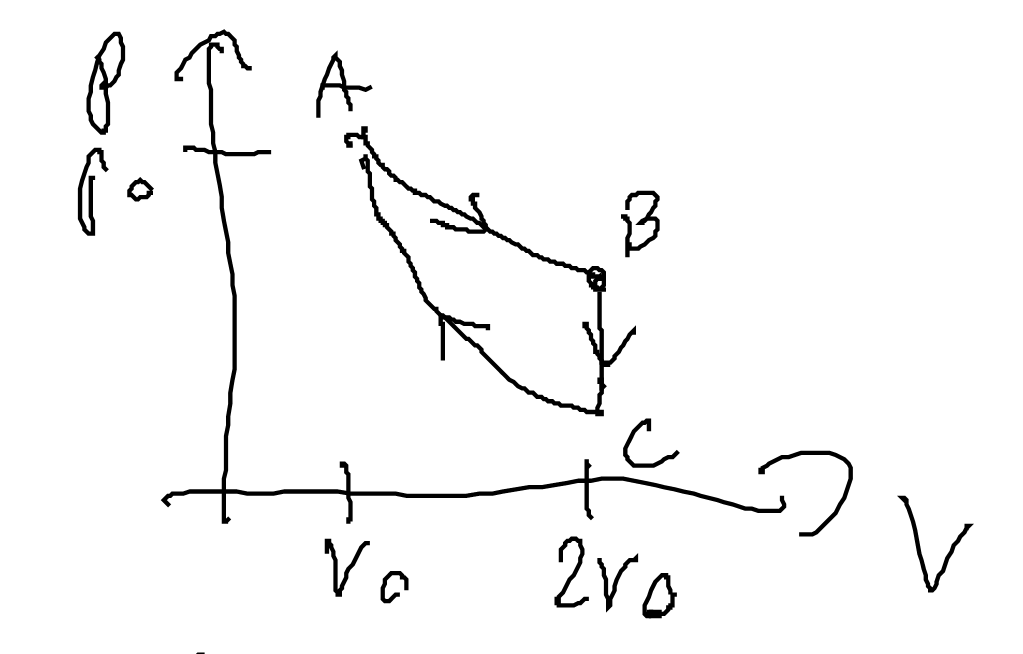
\includegraphics[width=0.4\textwidth]{zad4.PNG}
\end{center}

W procesie $A\rightarrow B$ stan gazu podąża wzdłuż krzywej zadanej równaniem $p^2 V = c$, gdzie $c$ pewna stała.
Praca wykonana nad gazem
$$
W_{A\rightarrow B} = -\int_{V_0}^{2 V_0} \sqrt{\frac{c}{V}}\,\t{d}V = -\sqrt{s} 2\left( \sqrt{2 V_0} - \sqrt{V_0}\right) = -2 p_0 V_0(\sqrt{2}-1).
$$
W przemianie izohorycznej praca jest równa zero:
$$
W_{B \rightarrow C} = 0.
$$
Z kolei w przemianie izotermicznej $p V = p_0 V_0$ więc:
$$
W_{C\rightarrow A} = - \int_{2V_0}^{V_0} \frac{p_0 V_0}{V}\, \t{d} V  = p_0 V_0 \ln 2.
$$
Ostatecznie całkowita praca wykonana nad gazem
 $$W = p_0 V_0 [\ln 2 -2(\sqrt{2}-1)] \approx -0.135 \,p_0V_0$$
 czyli to gaz efektywnie wykonał pracę.
%%%%%%%%%%%%%%%%%%%%%%%%%%%%%%%%%%%%%%%%%%%%%%%%%%
\newpage
%%%%%%%%%%%%%%%%%%%%%%%%%%%%%%%%%%%%%%%%%%%%%%%%%%
\zadanie
Oblicz pracę jaką wykona jeden mol gazu van der Waalsa, o równaniu stanu
$(p+\frac{a}{V^2})(V-b)=RT$
($a=0.138\,\rm{Jm}^3/\rm{mol}^2$, $b=31.8\,\rm{cm^3/mol}$)
przy izotermicznym i odwracalnym rozprężaniu od objętości $V_0=22.4\,\rm{dm}^3$
do objętości $2 V_0$ przy temperaturze $T=0\degree$C.
Przyjmij R = 8.31 J/(mol K).
Czy gaz doskonały rozprężając się w takich samych warunkach wykona większą pracę?

\vskip 10pt
\textbf{Rozwiązanie:}
Korzystając z równania stanu wyznaczamy zależność $p(V)$ dla procesu izotermicznego:
$$
p = \frac{R T}{V-b} - \frac{a}{V^2}.
$$
Stąd praca wykonana przez gaz:
$$
W = \int_{V_0}^{2 V_0} p \,\t{d}V = 
\int_{V_0}^{2V_0}\left(\frac{R T}{V-b} - \frac{a}{V^2}\right) = 
R T \ln \left(2 + \frac{b}{V_0 - b}\right) - \frac{a}{2V_0} = 1571.9\, \t{J}.
$$
Dla analogicznego procesu izotermicznego w przypadku gazu doskonałego mielibyśmy:
$$
W = \int_{V_0}^{2 V_0} p \,\t{d}V = 
\int_{V_0}^{2V_0}\left(\frac{R T}{V}\right) =  
RT \ln 2 =  1573\, \t{J},
$$
czyli nieznaczeni więcej. Z góry nie było oczywiste która praca będzie większa. Z jednej strony poprawka $b>0$ zwiększa ciśnienie w stosunku do gazu doskonałego a poprawka związana z $a>0$ zmniejsza.
%%%%%%%%%%%%%%%%%%%%%%%%%%%%%%%%%%%%%%%%%%%%%%%%%%
\newpage
%%%%%%%%%%%%%%%%%%%%%%%%%%%%%%%%%%%%%%%%%%%%%%%%%%
\zadanie
Równanie stanu paramagnetyka (np. w polu solenoidu) zapisać można jako:
\[  {\rm M}= C \frac{H}{T}, \]
gdzie $C$ - stała Curie, $H$ - natężenia pola magnetycznego, $T$- temperatura,
$\rm M$ - magnetyzacja, tj. moment magnetyczny $M$ w jednostce objętości (${\rm M}=M/V$).
Praca wykonana nad paramagnetykiem w polu magnetycznym
 (z wyłączeniem energii wzajemnej paramegantyk-solenoid) może być zapisana jako
 $\dbar W = -\mu_0 M dH$.
Znajdź pracę: 
\begin{itemize}
\item w przemianie izotermicznej przy zmianie momentu magnetycznego od $M_1$ do $M_2$
\item w przemianie dla której $H/T={\rm const}$, od $T_1$ do $T_2$. 
\end{itemize}

\vskip 10pt
\textbf{Rozwiązanie:}

\begin{itemize}
\item Z równania stanu mamy, 
\begin{equation}
	W = \int_{M_1}^{M_2} dW = - \mu_0 \int_{M_1}^{M_2} M dH.
\end{equation}	
Dla $T={\rm const}$, $dH = (T/C) dM$ więc 
\begin{equation}
	W = - \frac{1}{2} \frac{\mu_0 T}{C} \left(M_2^2 - M_1^2 \right).
\end{equation} 
\item W drugim przypadku $H/T$ jest stałe więc $M$ jest stałe. W takim razie 
\begin{equation}
	W = - \mu_0 M \int_{H_1}^{H_2} dH = - \mu_0 M (H_2 - H_1).
\end{equation}
$H_i$ możemy wyrazić przez $T_i$ jako $H_i = (M/C) T_i$ więc 
\begin{equation}
	W = - \frac{\mu_0 M^2}{C} (T_2 - T_1).
\end{equation}

\end{itemize}
%%%%%%%%%%%%%%%%%%%%%%%%%%%%%%%%%%%%%%%%%%%%%%%%%%
\newpage
%%%%%%%%%%%%%%%%%%%%%%%%%%%%%%%%%%%%%%%%%%%%%%%%%%
\zaddom
Stalowa szyna o przekroju poprzecznym $S = 10\,$cm$^2$ i długości $L = 10\,$m zmieniła temperaturę
z $20^\circ$C do $40^\circ$C.
\begin{enumerate}
\item Oszacuj o ile wzrosła długość szyny
\item Jakie siły powinny działać na końce szyny, aby przywrócić jej początkową długość? \\
      Czy wartość tych sił zależy od długości szyny?
\end{enumerate}
Przyjmij, że dla stali: współczynnik liniowej rozszerzalności cieplnej wynosi $\alpha = 1.2\cdot 10^{-5}\,$K$^{-1}$,
zaś moduł Younga wynosi $\displaystyle E = \frac{\Delta p}{\Delta L/L} = 200\,$GPa.

\vskip 10pt
\textbf{Rozwiązanie:}

Z definicji:
\begin{enumerate}
\item $\Delta L = L \alpha \Delta T = 2.4 \cdot 10^{-3}\, {\rm m}$,
\item $F = S \Delta p = S E \alpha \Delta T = 4.8 \cdot 10^4\, {\rm N}$.
\end{enumerate}
%%%%%%%%%%%%%%%%%%%%%%%%%%%%%%%%%%%%%%%%%%%%%%%%%%
\newpage
%%%%%%%%%%%%%%%%%%%%%%%%%%%%%%%%%%%%%%%%%%%%%%%%%%
\zaddom
Jeden mol gazu van der Waalsa ($a=0.138\,\rm{Jm}^3/\rm{mol}^2$, $b=31.8\,\rm{cm^3/mol}$)
utrzymywany jest pod stałym ciśnieniem normalnym w pojemniku o ściankach adiabatycznych, zamkniętym tłokiem,
wypełniając początkowo objętość $V_0=22,4\,\rm{dm}^3$.
W wyniku przesunięcia tłoka objętość jego wzrosła dwukrotnie. Podaj temperturę początkową i końcową.  
Jaki byłby wynik tego typu ekspansji w przypadku gazu doskonałego?

\vskip 10pt
\textbf{Rozwiązanie:}
Z równania stanu możemy policzyć początkową temperaturę
\begin{equation}
	T_0 = \frac{V_0-nb}{nR}\left(p_0 + \frac{n^2 a}{V_0^2} \right), \qquad T_0 = \frac{V_0 p_0}{nR}.
\end{equation}
Z równania przemiany adiabatycznej możemy wyznaczyć końcową temperaturę
\begin{equation}
	T_1 = T_0 \left(\frac{V_1 - nb}{V_0 - nb} \right)^{nR/C_v}, \qquad T_1 = T_0 \left(\frac{V_1}{V_0} \right)^{nR/C_v}.
\end{equation}
Reszta to podstawienie wielkości.
%%%%%%%%%%%%%%%%%%%%%%%%%%%%%%%%%%%%%%%%%%%%%%%%%%

\end{document}
